\documentclass{article}
\usepackage[utf8]{inputenc}    % For UTF-8 character encoding
\usepackage[T1]{fontenc}       % For proper font encoding
\usepackage{lmodern}           % Improved font rendering
\usepackage{amsmath}   % For advanced mathematical formatting
\usepackage{amssymb}   % For mathematical symbols
\usepackage{geometry}  % Adjust page margins
\usepackage{enumerate} % For custom lists
\usepackage{xcolor}  % for coloring
\usepackage{amsthm}
\usepackage{pdfpages}
\newtheorem{theorem}{Theorem}[section]
\newtheorem{lemma}[theorem]{Lemma}
\newtheorem{corollary}[theorem]{Corollary}
\newtheorem{definition}[theorem]{Definition}
\usepackage{listings}  % for code listings

\lstset{frame=tb,
  language=C,
  aboveskip=3mm,
  belowskip=3mm,
  showstringspaces=false,   
  columns=flexible,
  basicstyle={\small\ttfamily},
  numbers=none,
  numberstyle=\tiny\color{gray},
  keywordstyle=\color{blue},
  commentstyle=\color{brown},
  stringstyle=\color{orange},
  breaklines=true,
  breakatwhitespace=true,
  tabsize=3
}
\geometry{top=1in, bottom=1in, left=1in, right=1in}

\begin{document}

\title{}
\author{Wang Xiyu}
\date{}
\maketitle
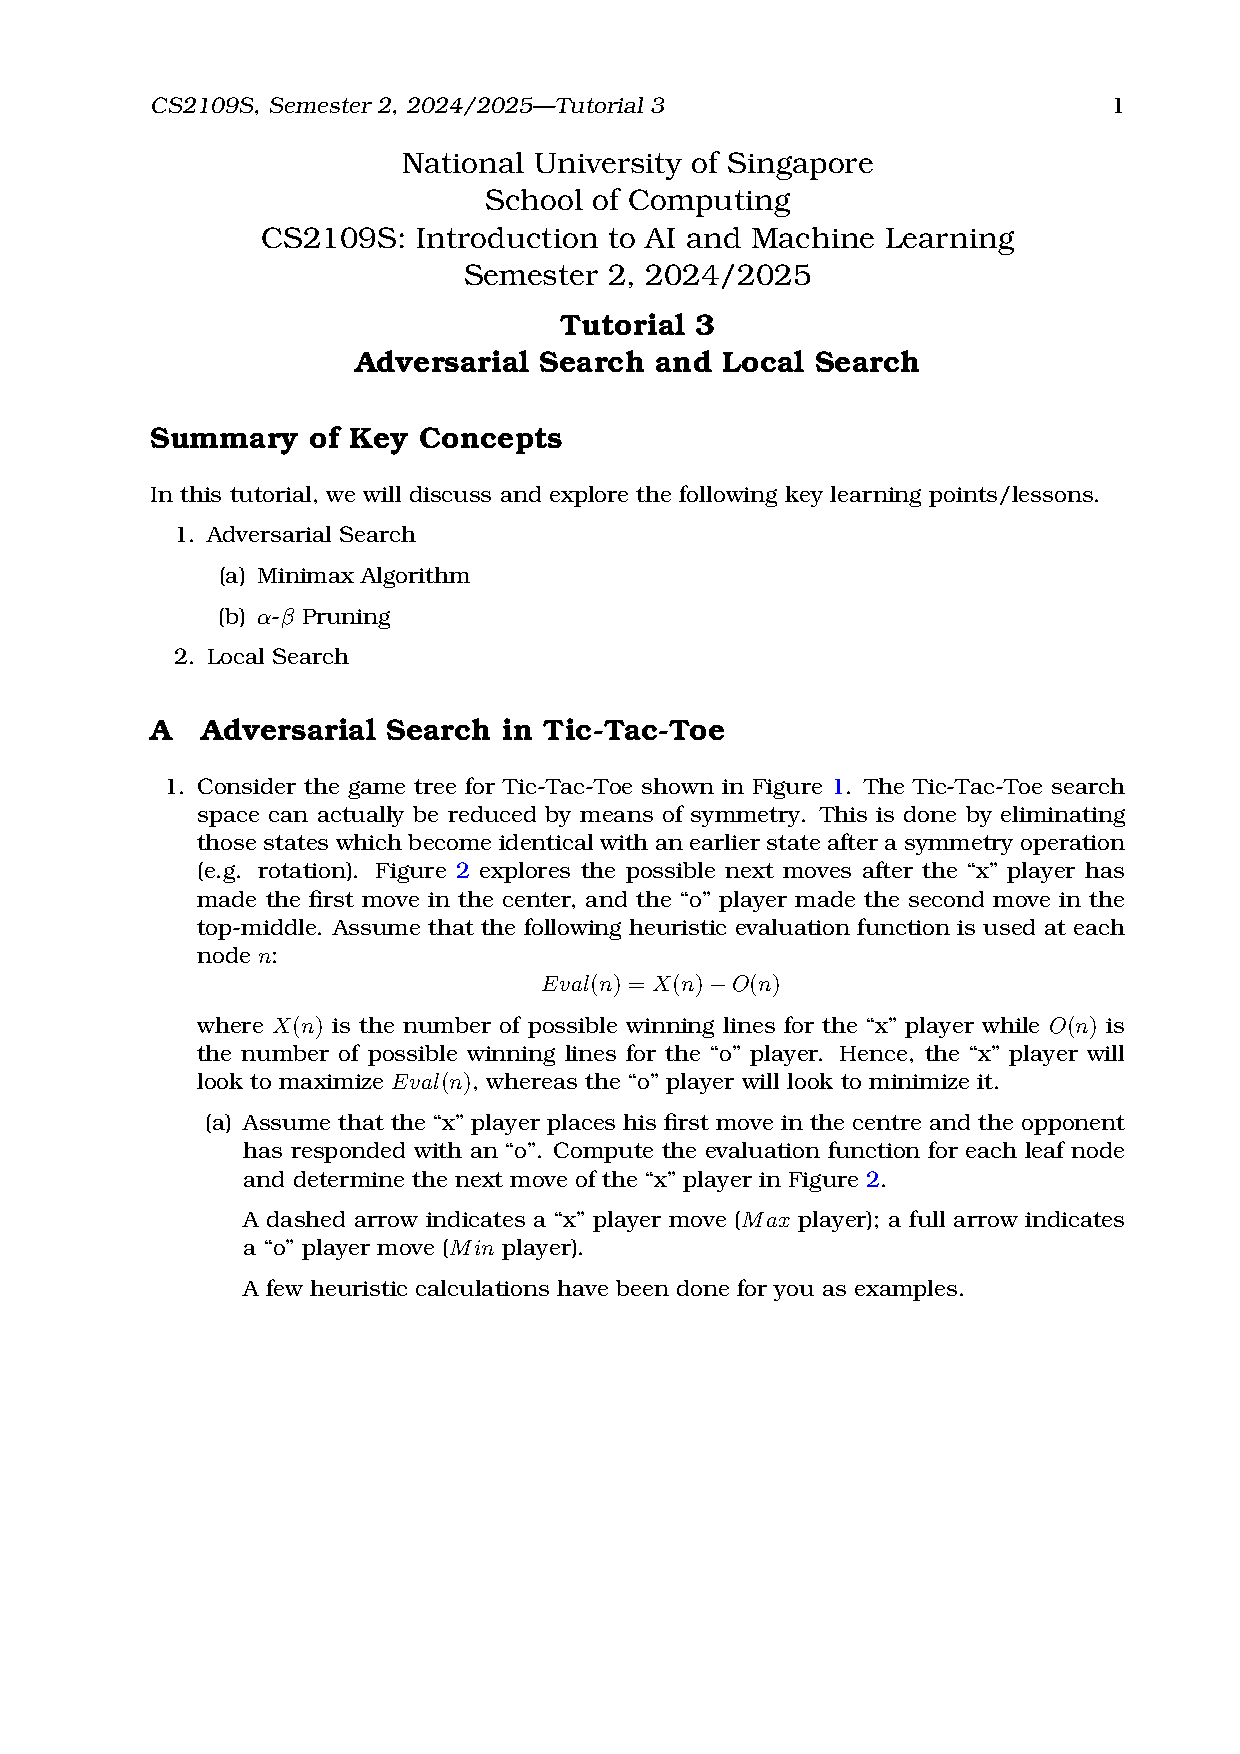
\includepdf[pages=1]{Tutorial3.pdf}
\section*{A}
\subsection*{a}
\[Eval(n) = X(n) - O(n)\]
\* Winning line here means potential wining combinations for one side:

\includepdf[pages=2]{Tutorial3.pdf}
\includepdf[pages=3]{Tutorial3.pdf}
\includepdf[pages=4]{Tutorial3.pdf}
\section*{B}
\subsection*{a}

\includepdf[pages=5]{Tutorial3.pdf}


\section*{Complexity analysis of Minimax and alpha beta pruning optimization}
Solve the recurrence relation with respect to the search depth $n$:
\[T(n)\]



\end{document}
